\documentclass{article}
\usepackage[pdftex]{graphicx,color}
\usepackage[T1]{fontenc}
\usepackage{lmodern}
\usepackage{amsmath}
\usepackage{amsfonts}
\usepackage{subcaption}
\usepackage{textpos}
\usepackage{setspace}


% use a larger page size; otherwise, it is difficult to have complete
% code listings and output on a single page
\usepackage{fullpage}

% have an index. we use the imakeidx' replacement of the 'multind' package so
% that we can have an index of all run-time parameters separate from other
% items (if we ever wanted one)
\usepackage{imakeidx}
\makeindex[name=prmindex, title=Index of run-time parameter entries]
\makeindex[name=prmindexfull, title={Index of run-time parameters with section names\label{sec:index}}]

% be able to use \note environments with a box around the text
\usepackage{fancybox}
\newcommand{\note}[1]{
{\parindent0pt
  \begin{center}
    \shadowbox{
      \begin{minipage}[c]{0.9\linewidth}
        \textbf{Note:} #1
      \end{minipage}
    }
  \end{center}
}}

% use the listings package for code snippets. define keywords for prm files
% and for gnuplot
\usepackage{listings}
\lstset{
  language=C++,
  showstringspaces=false,
  basicstyle=\small\ttfamily,
  columns=fullflexible,
  keepspaces=true,
  frame=single,
  breaklines=true,
  postbreak=\raisebox{0ex}[0ex][0ex]{\hspace{5em}\ensuremath{\color{red}\hookrightarrow\space}}
}
\lstdefinelanguage{prmfile}{morekeywords={set,subsection,end},
                            morecomment=[l]{\#},escapeinside={\%\%}{\%},}
\lstdefinelanguage{gnuplot}{morekeywords={plot,using,title,with,set,replot},
                            morecomment=[l]{\#},}


% use the hyperref package; set the base for relative links to
% the top-level \dftfe directory so that we can link to
% files in the \dftfe tree without having to specify the
% location relative to the directory where the pdf actually
% resides
\usepackage[colorlinks,linkcolor=blue,urlcolor=blue,citecolor=blue,baseurl=../]{hyperref}

\makeatletter
\renewcommand\paragraph{\@startsection{paragraph}{4}{\z@}%
            {-2.5ex\@plus -1ex \@minus -.25ex}%
            {1.25ex \@plus .25ex}%
            {\normalfont\normalsize\bfseries}}
\makeatother
\setcounter{secnumdepth}{4} % how many sectioning levels to assign numbers to
\setcounter{tocdepth}{4}    % how many sectioning levels to show in ToC


\newcommand{\biodeg}{\textsc{BioDeg}}

\begin{document}

\definecolor{dark_grey}{gray}{0.3}
\definecolor{biodeg_blue}{rgb}{0.0,0.39,0.76}

%LINE 1%
{
\renewcommand{\familydefault}{\sfdefault}

\pagenumbering{gobble}

%COLOR AND CODENAME BLOCK%
\begin{center}
\resizebox{\textwidth}{!}{\colorbox
{biodeg_blue}{\fontfamily{\rmdefault}\selectfont \textcolor{yellow} {
\hspace{0.1in}\biodeg{}\hspace{0.1in}
}}}
\\[12pt]
{\Large Biodegradation and Corrosion Simulation using Finite Element}
\end{center}

%MAIN PICTURE%
%\begin{textblock*}{0in}(0.5in,0.3in)
%\begin{center}
%\vspace{1em}
%\includegraphics[scale=0.35]{N2.png}
%\hspace{5em}
%\end{center}
%\end{textblock*}

%USER MANUAL%
\color{dark_grey}
\vspace{1.0em}
\hfill{\Huge \fontfamily{\sfdefault}\selectfont User Manual \\
\raggedleft \huge \fontfamily{\sfdefault}\selectfont Version
0.8 %VERSION-INFO%
\\\large(generated \today)\\
\vspace{1.5em}
{\Large Mojtaba Barzegari\,\\Liesbet Geris\\}
\vspace{1.0em}
\large
%\noindent with contributions by: \\
%    {\Large Krishnendu Ghosh\\}
\vspace{1.0em}
}
%WEBSITE%
\null
\vspace{17em}

{\noindent
{\fontfamily{\sfdefault}\selectfont \href{https://github.com/mbarzegary/BioDeg-UI}{BioDeg website}}
}

\begin{textblock*}{0in}(4.8in,-0.5in)

\includegraphics[height=0.5in]{KUL.png}
\end{textblock*}

%LINE%
{\noindent
\color{dark_grey}
\rule{\textwidth}{2pt}
}

}
Copyright (c) 2019-2021 University of Leuven and \hyperref[sec:authors]{BioDeg authors}.
\pagebreak
\pagenumbering{arabic}

\pagebreak

\onehalfspacing

\tableofcontents

\pagebreak

\section{Introduction}
\label{sec:intro}
\biodeg{} is an open-source software written in FreeFEM (a domain-specific language for finite element programming), C++, and Python for modeling the degradation of metallic biomaterials and simulating the biodegradation behavior of medical devices, implants, and scaffolds in corrosion experiments. It can handle any geometry of desire and supports parallel computing to simulate large-scale models.

\subsection{Authors}
\label{sec:authors}
\biodeg{} is developed by the \href{http://www.biomech.ulg.ac.be/}{Biomechanics Research group at KU Leuven and University of Liege}. The code is currently maintained by its principal developer, 
who manages the development of the mathematical models and the core functionalities. 

\paragraph*{Principal developer}
\begin{itemize}
	\item Mojtaba Barzegari (University of Leuven, Belgium)
\end{itemize}

\paragraph*{Previous Contributors}
\begin{itemize}
	\item Yann Guyot (University of Liege, Belgium)
	\item Piotr Bajger (University of Oxford, UK)
\end{itemize}

\paragraph*{Mentor}
\begin{itemize}
	\item Liesbet Geris (University of Leuven, Belgium)
\end{itemize}

\paragraph*{Chemist contributors}
(who has helped to validate the models)
\begin{itemize}
	\item Sviatlana V. Lamaka (Helmholtz-Zentrum Hereon, Gremany)
	\item Di Mei (Zhengzhou University, China)
	\item Cheng Wang (Helmholtz-Zentrum Hereon, Gremany)
\end{itemize}

\subsection{Acknowledgments}
The development of \biodeg{} open-source code is financially supported by the Prosperos project, funded by the Interreg VA Flanders – The Netherlands program, CCI grant no. 2014TC16RFCB046 and by the Fund for Scientific Research Flanders (FWO), grant G085018N. The developers also acknowledge support from the European Research Council under the European Union's Horizon 2020 research and innovation programmen, ERC CoG 772418.

\subsection{Referencing \biodeg{}}

Please refer to \href{https://github.com/mbarzegary/BioDeg}{\biodeg{} repository}, section "Publications and referencing" to properly cite the use of 
\biodeg{} in your scientific work. 


\section{Useful background information}
\label{sec:background}
You may refer to the following articles for a background of the methods and algorithms implemented in \biodeg. \\

%\noindent 1. P. Motamarri, M.R. Nowak, K. Leiter , J. Knap, V. Gavini, Higher-order adaptive finite-element methods for Kohn-Sham density functional theory, \emph{J. Comput. Phys.} 253, 308-343 (2013).\\
% 
%\noindent 2. P. Motamarri, V. Gavini, Subquadratic-scaling subspace projection method for large-scale Kohn-Sham DFT calculations using spectral finite-element discretization, \emph{Phys. Rev. B} 90, 115127 (2014).\\

\noindent In addition, below are some useful references on finite element method and some online resources that provide a background of finite elements and their application to the solution of partial differential equations.\\





\section{Installation}
\label{sec:installation}
Installing \biodeg{} is a straightforward procedure. You need to install a couple of prerequisites and download and run \biodeg{}; that's all you need to do. But for advanced users, it might be necessary or more interesting to build everything from scratch to have more control over customizing features and improving performance. As a result, we have provided 2 sets of instructions, one for easy installation using the compiled binaries and one for building things from the source codes. The installation instructions are provided for Linux and Windows operating systems, but the procedure should be very similar for macOS. 

It is possible to use \biodeg{} without the user interface (UI) if this scenario is required by the user (like for running it on a super-computer). The core of \biodeg{} is written in FreeFEM, so in this case, all you need to do is to install/build FreeFEM and the required libraries, and then, clone the \href{https://github.com/mbarzegary/BioDeg}{\biodeg{} core repository} and run the code according to the provided instruction in the README file of the repository.

The \biodeg{} UI contains all the bundles for pre-processing and post-processing simulation input/results. These features are being hosted on their own repositories (), but with obtaining the user interface, you can have them all together. If you choose to use \biodeg{} without the user interface and still want to use the provided script for pre/post-processing, you may need to obtain them separately.

For building the source codes, we assume standard tools and libraries like CMake, compilers (for C, C++ and Fortran), and MPI libraries are pre-installed on your machine. If you are going to build \biodeg{} and required dependencies on a super-computer or cluster, you should notice that most high-performance computers would have the latest version of these compilers and libraries in the default environment.

\subsection{Easy installation}

The simplest way to install and run \biodeg{} is via the pre-built binaries you can download from GitHub. The same principle applies to prerequisites, which is in this case FreeFEM only. So, following these steps will install \biodeg{} on your machine:

\begin{enumerate}
\item
Download FreeFEM installer for the platform you use and install it. You can find the {.exe} installer for Windows and the {.deb} installer for Linux (Ubuntu) in the \href{https://github.com/FreeFem/FreeFem-sources/releases}{Release page of FreeFEM repository}. You will find these files under the Assets section of the latest (or any other version). Execute the download file and follow the installation procedure appearing on your screen.
\item
Download \biodeg{} tarballs for your preferred platform (Windows or Linux) from the \href{https://github.com/mbarzegary/BioDeg-UI/releases}{Release page of \biodeg{} repository}. This is indeed the \biodeg{} UI bundle that contains the \biodeg{} core, the user interface, the pre-processor, and the post-processor.
\item
Extract the downloaded tarball (zip) file and execute \verb|runBioDeg.cmd| in Windows or \verb|runBioDeg.sh| in Linux. By doing this, you see the \biodeg{} interface showing up on the screen.
\end{enumerate}




\subsection{Advanced installation for improved performance/flexibility}

Building \biodeg{} and required libraries from source code will increase the performance since the program and the libraries will get optimized for the platform in which they are going to run. Moreover, this enables users to customize the software in the way they want. Additionally, this is an inevitable aspect if you are going to use \biodeg{} for development purposes or you want to contribute to it.

\subsubsection{Compiling and installing external libraries}

\paragraph{PETSc and Qt}

\biodeg{} uses \href{https://petsc.org/release/}{PETSc} for parallel computing. You may choose to build a customized version of PETSc or use the version that comes with FreeFEM. The version that is bundled with FreeFEM has the following build configuration:

\begin{verbatim}
--with-debugging=0 COPTFLAGS="-O3 -mtune=native" CXXOPTFLAGS="-O3 -mtune=native" 
FOPTFLAGS="-O3 -mtune=native" --with-cxx-dialect=C++11 --with-ssl=0 --with-x=0 
--with-fortran-bindings=0 --with-cc=/usr/ --with-scalar-type=complex
--with-blaslapack-include= --with-blaslapack-lib="-llapack -lblas"
--with-scalapack --with-metis --with-ptscotch --with-suitesparse --with-suitesparse-lib=
"-Wl, -lumfpack -lklu -lcholmod -lbtf -lccolamd -lcolamd -lcamd -lamd -lsuitesparseconfig"
--with-mumps --with-parmetis --with-tetgen --download-slepc --download-hpddm PETSC_ARCH=fc
\end{verbatim}

You may need to build your own version if this configuration is not suitable for you. You can find the instruction for building custom version of PETSc \href{https://petsc.org/release/install/}{here}.

\biodeg{} UI is developed using \href{https://www.qt.io/}{Qt} so it should be installed on your system if you want to compile \biodeg{} UI. You can find the installation instruction for various platforms \href{https://doc.qt.io/qt-5/gettingstarted.html}{here}.

\paragraph{FreeFEM}

The full build documentation of FreeFEM is available \href{https://doc.freefem.org/introduction/installation.html}{here}, but the following steps is what you need to do to build it on any platform. By default, FreeFEM downloads and builds PETSc during the build process.

\begin{enumerate}
\item Install required prerequisites
\begin{verbatim}
$ sudo apt-get install cpp freeglut3-dev g++ gcc gfortran m4 make patch pkg-config
  wget python unzip liblapack-dev libhdf5-dev libgsl-dev autoconf automake 
  autotools-dev bison flex gdb git cmake
$ sudo apt-get install mpich
\end{verbatim}

\item Make a new directory for FreeFEM and navigate to it
\begin{verbatim}
$ cd
$ mkdir FreeFEM
$ cd FreeFEM/
\end{verbatim}

\item Clone the source code repository and navigate to the downloaded directory
\begin{verbatim}
$ git clone https://github.com/FreeFem/FreeFem-sources.git
$ cd FreeFem-sources/
\end{verbatim}

\item Generate the configure scripts
\begin{verbatim}
$ autoreconf -i
\end{verbatim}

\item Run the configure script to specify build options, including the location to install the program
\begin{verbatim}
$ ./configure --enable-download --enable-optim 
  --prefix=/home/<your_profile>/FreeFEM/freefem-install
\end{verbatim}

\item Download the source code of 3rd-party libraries
\begin{verbatim}
$ ./3rdparty/getall -a
\end{verbatim}

\item Build PETSc and all the 3rd-party libraries
\begin{verbatim}
$ cd 3rdparty/ff-petsc/
$ make petsc-slepc
\end{verbatim}

\item Navigate back and reconfigure the build
\begin{verbatim}
$ cd -
$ ./reconfigure
\end{verbatim}

\item Build the source code of FreeFEM using 4 parallel processes (or any other number you like
\begin{verbatim}
$ make -j4
\end{verbatim}

\item Check the build by running some examples
\begin{verbatim}
$ make -j2 check
\end{verbatim}

\item Install the built binaries to the specified directory
\begin{verbatim}
$ make install
\end{verbatim}

\item Navigate to the installation location and run FreeFEM
\begin{verbatim}
$ cd ../freefem-install/
$ cd bin/
$ ./FreeFem++
\end{verbatim}

\item Navigate to the home directory and add FreeFEM to the PATH variable in the \verb|.bashrc`| file
\begin{verbatim}
$ cd
$ nano .bashrc
\end{verbatim}
and add \verb|export PATH=$PATH:/home/<your_profile>/FreeFEM/freefem-install/bin| to the end of the file and save (press \textit{Ctrl+X} and then \textit{Y}).

\end{enumerate}

After doing this, you should be able to run FreeFEM. Start a new terminal and run \verb|FreeFem++| and \verb|FreeFem++-mpi|. See ing no error in the output means that you have successfully installed it.

\subsubsection{Building and installing \biodeg{}} \label{sec:build_biodeg}

Since \biodeg{} UI is developed using Qt, compiling the source files is quite straightforward. Upon installing Qt on your machine, clone the \href{https://github.com/mbarzegary/BioDeg-UI}{\biodeg{} UI repository} and follow one of the following scenarios to build it. 

\paragraph{Build \biodeg{} UI using Qt Creator IDE}

This is the simplest technique to build the program, and it has a similar procedure for all the supported platforms. Qt Creator is the default IDE for Qt development, so it is automatically installed along with Qt. Simply open the Qt project file (\verb|CMakeLists.txt|) in Qt Creator (by executing \verb|qtcreator CMakeLists.txt| or selecting \textit{File->Open Project} from the IDE) and build the project (by pressing \textit{Shift+B}).

\paragraph{Build \biodeg{} UI using Qt tools}

Building the source files using CMake is also quite simple. Navigate to the source files directory (the cloned repository) and run the following commands (this assumes that you have already added Qt \verb|bin| directory to the `PATH` variable so that the CMake script can find Qt libraries and binaries):

\begin{verbatim}
$ mkdir build
$ cd build
$ cmake ..
$ make
\end{verbatim}

In Windows, you may need to call the correct build system installed along with Qt. For example, by assuming that you have installed the MinGW integration for Qt, the \verb|make| command should be written as \verb|mingw32-make|. Moreover, in this case, you need to call CMake with a suitable generator, so the \verb|cmake| command should be replaced by something like \verb|cmake -G "MinGW Makefiles" ..| (don't forget to insert the double dots).

After doing this, you can find the \biodeg{} UI executable in the build (or bin) directory and run it by executing \verb|./BioDeg| in Linux or \verb|.\BioDeg.exe| in Windows.

\subsubsection{Testing \biodeg{}}

The testing module of \biodeg{} is developed using \href{https://github.com/google/googletest}{Google Testing framework}. The tests cover some basic and advanced evaluation of the functionality of FreeFEM installation and \biodeg{}-core, so running them may take several minutes to complete. 

After building \biodeg{} using the process mentioned in Section~\ref{sec:build_biodeg}, you can run the tests simply by executing the following command (in the build directory):

\begin{verbatim}
$ make test
\end{verbatim}
which can be \verb|mingw32-make test| in Windows. You can review the results upon completion of all the tests. In a healthy installation of FreeFEM and \biodeg{}, all tests should pass successfully. 

\section{Running \biodeg}
\label{sec:run}
After installing/compiling \biodeg{} as described in Section~\ref{sec:installation}, we are ready to run it. There are 2 ways to run \biodeg{} simulations: 1) using the UI to configure and execute \biodeg{}, or 2) running \biodeg{} directly from command line and provide simulation parameters via command line arguments. Moreover, in a hybrid approach, the UI can be used to configure and generate the command for method \#2, which can be useful in which you want to configure the simulation only and run it later in another environment like on a super-computer or cluster.

The UI can be run simply by double clicking on the \verb|BioDeg-UI.exe| in Windows or by executing \verb|./BioDeg-UI| in Linux. For running \biodeg{} directly, one need to execute the following command:
\begin{verbatim}
$ mpirun -n N FreeFem++-mpi BioDeg-core/src/main.edp <command line args>
\end{verbatim}
in which N defines the number of MPI processes to be used. The full list of command line arguments can be found in Section \hyperref[sec:index]{Index}.

In order to clarify and demonstrate the procedure of performing simulations using \biodeg{}, 2 step-by-step examples are provided in Section~\ref{sec:config}, showing how to configure and run simulations with and without the UI. Moreover, a third example shows how to combine these approaches and use the UI to generate the execution command. The mesh files needed to run these examples can be found in the \verb|demo| directory. Additionally, Section~\ref{sec:postprocess} provides some guidelines on the postprocessing of the  \biodeg{} simulation results. 

\subsection{Configuring the simulation} \label{sec:config}


\subsubsection{Example 1 - degradation of a simple screw}\label{sec:example1}

Let us consider the first example given in the \verb|demo| directory, where we simulate the biodegradation of a small screw. The size of the screw was chosen to be very small intentionally to make the simulation shorter such that the user can see the effect of the degradation much faster. The input mesh file is named \verb|screw.mesh|. For this example, we use the \biodeg{}-UI interface to perform the simulation. 

Let's conduct the first simulation with most of the parameters left with their default values. Run the user interface, and mark \menu[,]{Geometry \& Mesh, Import external mesh}. Then click the browse button in front of the ``File'' box (\menu[,]{Geometry \& Mesh, Import mesh, File}), navigate to the \verb|demo| directory, and select the \verb|screw.mesh| file. The path should be inserted in the ``File'' box. Selecting appropriate label numbers of the external mesh is very crucial in \biodeg{}, so you should always check the labels before importing the mesh. One of the best tools to do this is GMSH, in which you can view the labels of mesh files by opening the mesh and navigating to \menu[,]{Tools, Visibility}. Doing this on the \verb|screw.mesh| shows that the label number of the scaffold is 2 while the medium has a label number of 1 (Fig.~\ref{fig:gmsh_label}). So, we need to switch the default labels by selecting 2 for the scaffold (\menu[,]{Geometry \& Mesh, Import mesh, Scaffold label}) and 1 for the medium (\menu[,]{Geometry \& Mesh, Import mesh, Medium label}).

\begin{figure}[h]
\center 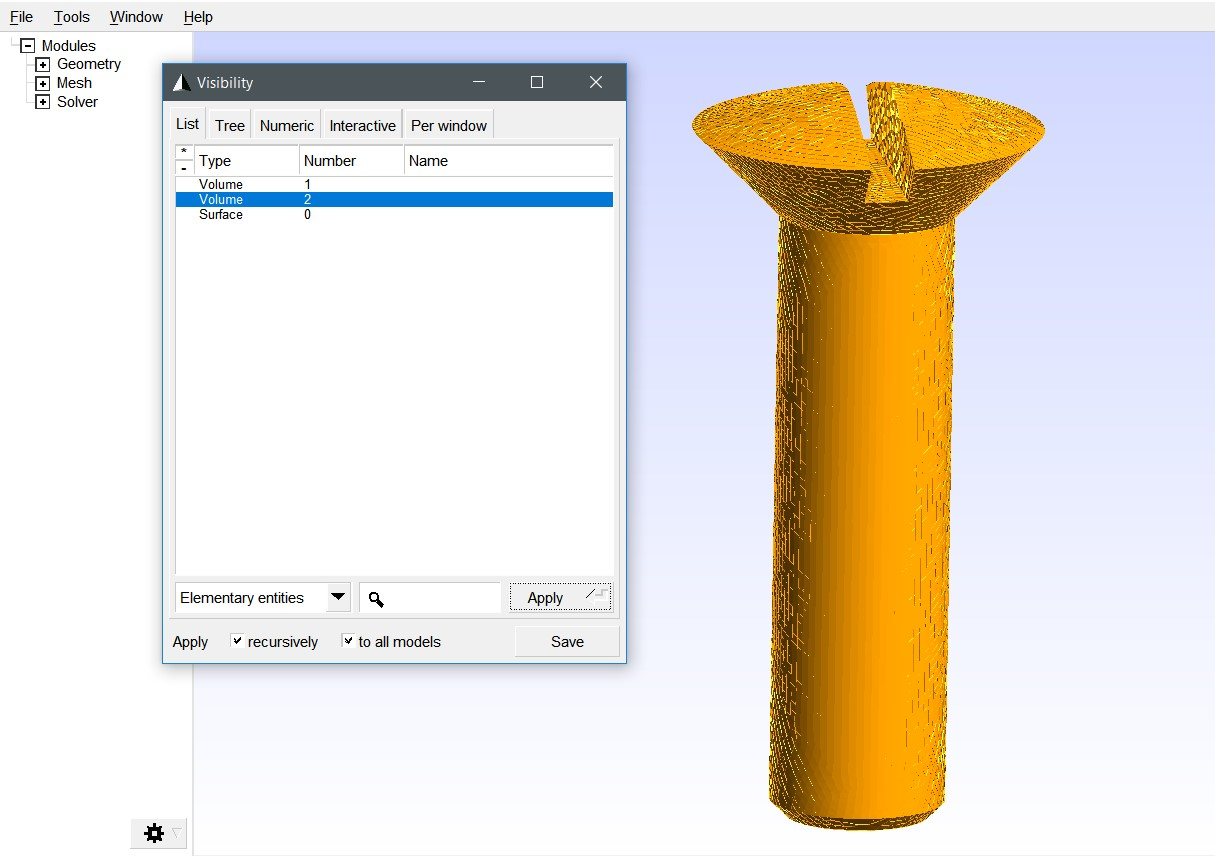
\includegraphics[width=15cm]{gmsh_label}
\caption{Using GMSH to read the labels of the mesh} \label{fig:gmsh_label}
\end{figure}

We need to enable the VTK output if we want to see the graphical output of the simulations. Navigate to \menu[,]{Output, Output options, Write VTK output} and mark it. You should also specify the output directory by clicking on the browse button in front of the ``Output directory'' (\menu[,]{Output, Output options, Output directory}) and select a directory of desire. 

That was all we needed to do to setup a simulation in \biodeg{}, and you can start the simulation by pressing the \menu[,]{Run simulation} button located in the middle of the main window. There are lot more parameters we can deal with (see Section \hyperref[sec:index]{Index}), but the input and output are the most essential ones. 

Although you can start the simulation of this example right now, there is a couple of more things you may want to change:

\begin{itemize}
\item
In \biodeg{}, simulations are by default carried out in parallel using domain decomposition, meaning that the simulation is distributed among available computing nodes. If you are running \biodeg{} on your local machine, you may need to adjust the parallel computing settings. Navigate to \menu[,]{Solver, Parallel computing, Enable parallel computing} and disable it if you don't want to parallelize the simulation. If you want to continue with parallelization enabled (default behavior), you may need to adjust the number of parallel processes to match the number of free CPU cores you have on your machine. You can change it in \menu[,]{Solver, Parallel computing, CPU/MPI cores}. 
\item
The default degradation rate is quite fast, so you may want to decrease it by reducing the diffusion coefficient of the metallic ions (please refer to ``Theory Guide'' if you want to know more about diffusion controls the rate of degradation). The default diffusion rate is the value we have estimated for saline solutions, which leads to a high rate of corrosion. You can apply this it by changing the value in \menu[,]{Material \& BCs, Reaction-diffusion properties, Metal ion diffusion coefficient} and reduce it to something like $0.0005$, which is its order when it comes to buffered solutions and simulated body fluids.
\item
The results write interval, implying how frequently you want to store the results, affects the resource consumption (which is storage in this case) and the quality of the graphical postprocessing. So, you should configure this carefully to keep the balance of the quality and resource consumption. The default save interval is $0.25$ hours of simulation time, but you can change it in \menu[,]{Output, Output options, Save results every ... hours}. For this simulation, since the screw geometry is small and degrades very fast, you can reduce this to $0.1$ to be able to see the degradation steps better.
\item
Final simulation time does not affect the simulation progress, but it is always a good practice to adjust it, enabling us to track the progress of the simulation better and avoid wasting resources (both computing power and storage). The default simulation time is 21 hours, but you can reduce it in \menu[,]{Solver, Time control, Final simulation time (hour)}. For this simulation, you can reduce it to 2.
\end{itemize}

After running the simulation (by pressing the \menu[,]{Run simulation} button), you can view the progress of the simulation on the UI, showing you how many steps have been taken and how much material degradation has happened (Fig~\ref{fig:screw_gui}). The UI also shows you the details info of the size of the problem, including the degrees of freedom (DOF) of each equation and the number of elements, as well as the number of DOFs for each sub-domain after mesh partitioning (for parallel computing). 

\begin{figure}[h]
\center 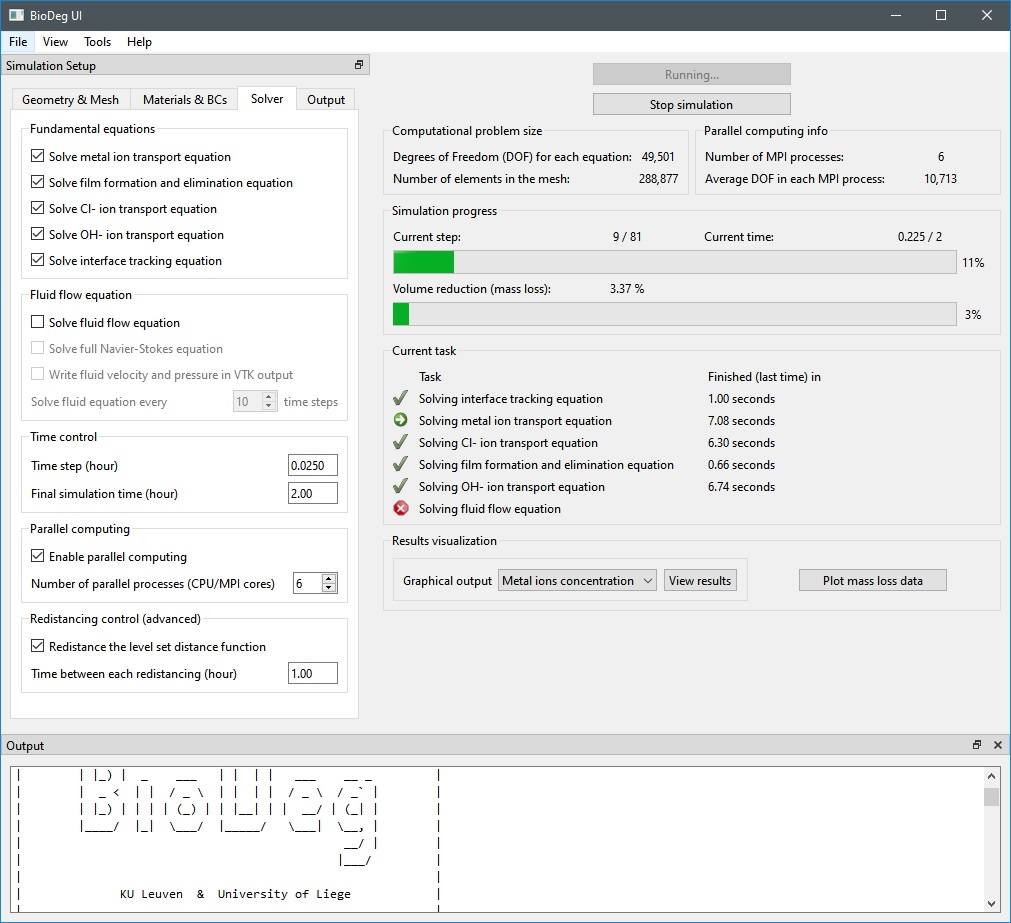
\includegraphics[width=12cm]{screw_gui}
\caption{\biodeg{}-UI running the screw degradation example.} \label{fig:screw_gui}
\end{figure}

Running this simulation leads to the results demonstrated in Fig.~\ref{fig:screw_degradation}, showing how the screw degrades. For more information on how to postprocess the results, please refer to the postporcessing section.

\begin{figure}[h]
\center 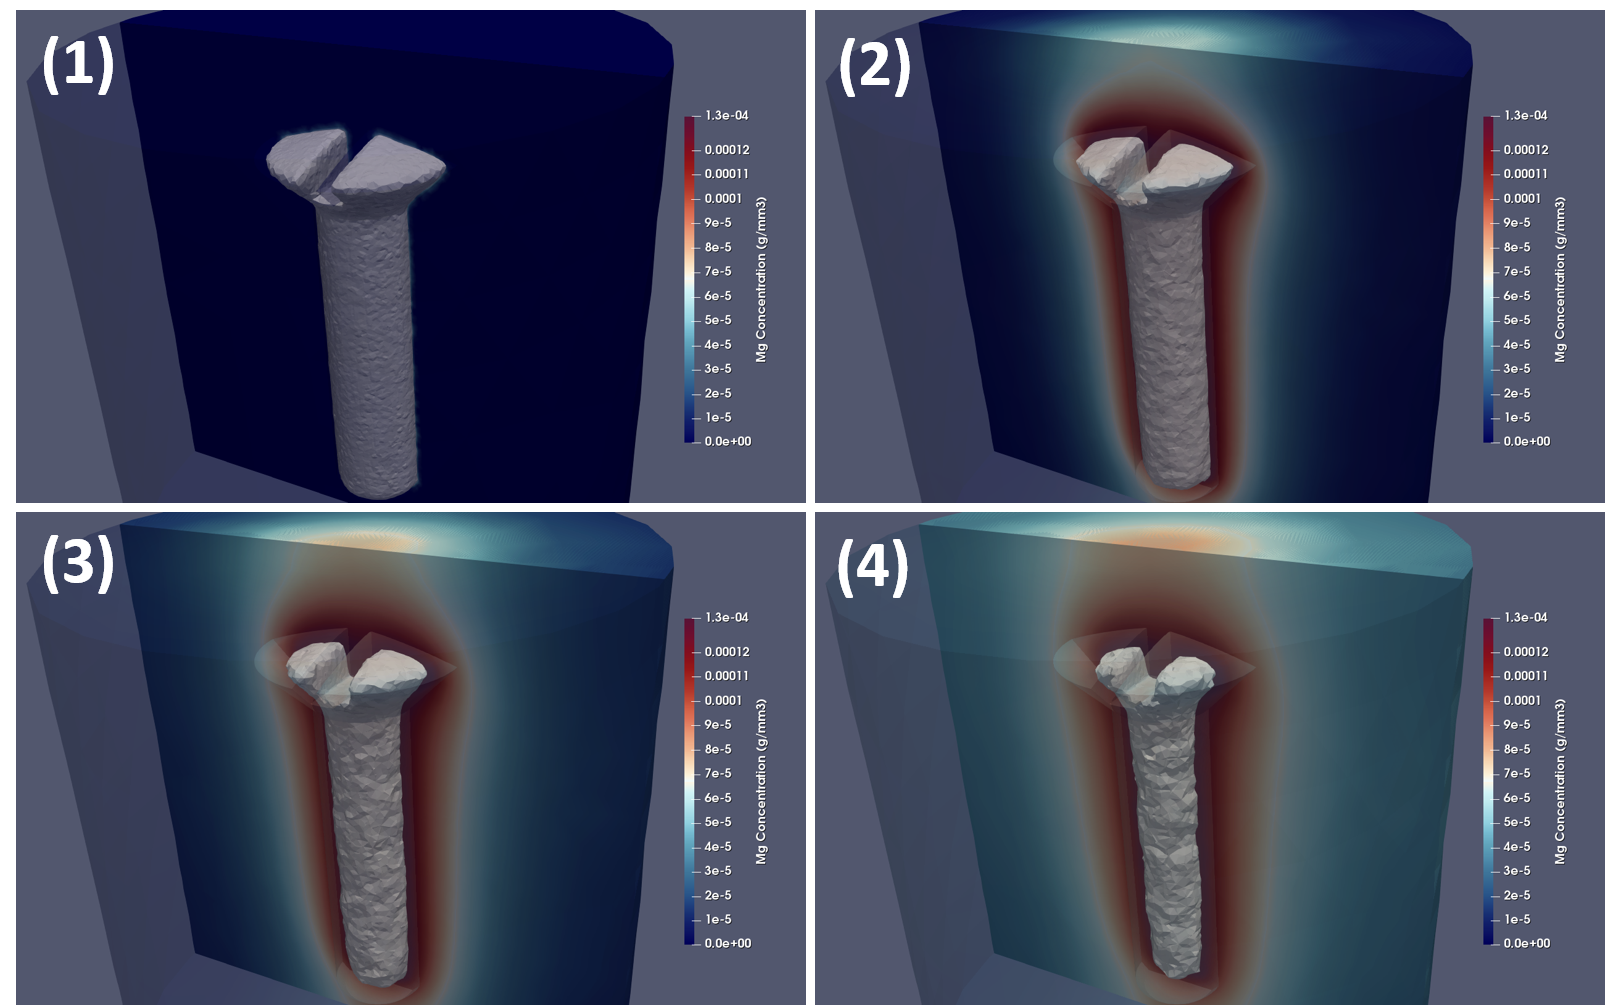
\includegraphics[width=15cm]{screw_degradation}
\caption{Simulation of the biodegradation of a simple screw, showing how the material is released and how the implant degrades.} \label{fig:screw_degradation}
\end{figure}


\subsubsection{Example 2 - degradation of a helical shape (Biomech logo)}\label{sec:example2}

In the second example, we want to run a heavier biodegradation simulation (with $\num{1484412}$ elements and a DOF of $\num{254157}$ for each equation), so let's do it by calling \biodeg{} directly on the command line. This approach can be taken on remote clusters and HPC environments to run \biodeg{} on hundreds or thousands of computing nodes. 

The model in this example has a helical shape, which is actually the logo of the lab in which \biodeg{} has been developed. The input mesh file is called \verb|biomech_logo.mesh| and is located in the \verb|demo| directory. Similar to the previous example, we try to use the default value of parameters and only change the crucial ones. You should notice that the default value of parameters might be different between the core \biodeg{} and the UI, so it's always better to define them explicitly in the execution command. The default values of parameters can be checked in Section  \hyperref[sec:index]{Index}.

The main file of the \biodeg{} code is called \verb|main.edp|, and since it's a parallel code, we should run it with the \verb|mpiexec| command. So, calling the code with all the default parameters on 6 MPI cores can be done like this:
\begin{verbatim}
$ mpiexec -n 6 FreeFem++-mpi BioDeg-core/src/main.edp -v 0
\end{verbatim}

The \verb|-v 0| is added to suppress the messages that FreeFEM writes to the terminal, and it's recommended to include it on any call you make to \biodeg{}. Calling \biodeg{} like this does nothing for us, so let's complete the command by adding more configuration to it (remember that boolean values are passed by their integer equivalents, 0 for false and 1 for true):

\begin{itemize}
\item
Turn off the fluid flow simulation and ignore the convection effect: \verb|-solve_fluid 0|
\item
Indicate that we want to import an external mesh: \verb|-import_mesh 1|
\item
Specify the name of the mesh, located in the \verb|demo| directory: \verb|-mesh_file "demo/biomech_logo.mesh"|
\item 
Specify the labels of different regions, which are crucial parameters as discussed in previous example (Section~\ref{sec:example1}): \verb|-label_scaffold 3 -label_medium 4|
\item
You can lower the degradation rate a little bit if you like. You may run the simulation several times and see the effect of this parameter in action: \verb|-d_mg 0.005|
\end{itemize}

Adding all the above arguments forms the final execution command to run:
\begin{verbatim}
$ mpiexec -n 6 FreeFem++-mpi BioDeg-core/src/main.edp -v 0 -solve_fluid 0 -import_mesh 1 
-mesh_file "demo/biomech_logo.mesh" -label_scaffold 3 -label_medium 4 -d_mg 0.005
\end{verbatim}

The above command execute \biodeg{}, which writes its output to the terminal (Fig~\ref{fig:logo_terminal}) and stores the simulation results to the default directory called \verb|output| (make sure it exists before calling \biodeg{}). 

\begin{figure}[h]
\center 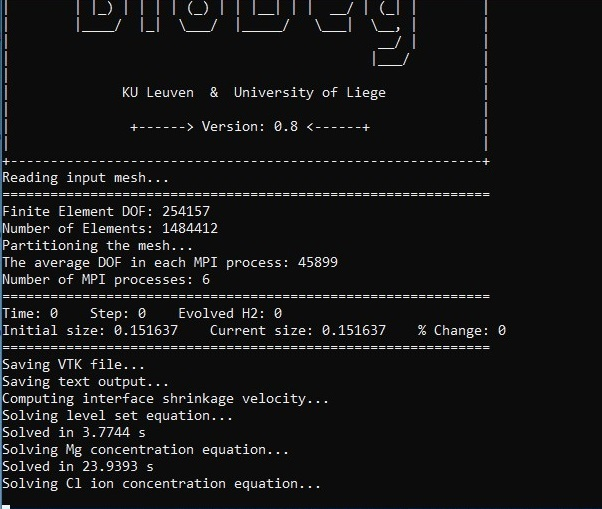
\includegraphics[width=10cm]{logo_terminal}
\caption{Output of \biodeg{} code for the logo example.} \label{fig:logo_terminal}
\end{figure}

The output of this simulation is shown in Fig~\ref{fig:logo_degradation}, which is postprocessed using the NVIDIA IndeX. Please refer to the postprocessing section to see how to do it.

\begin{figure}[h]
\center 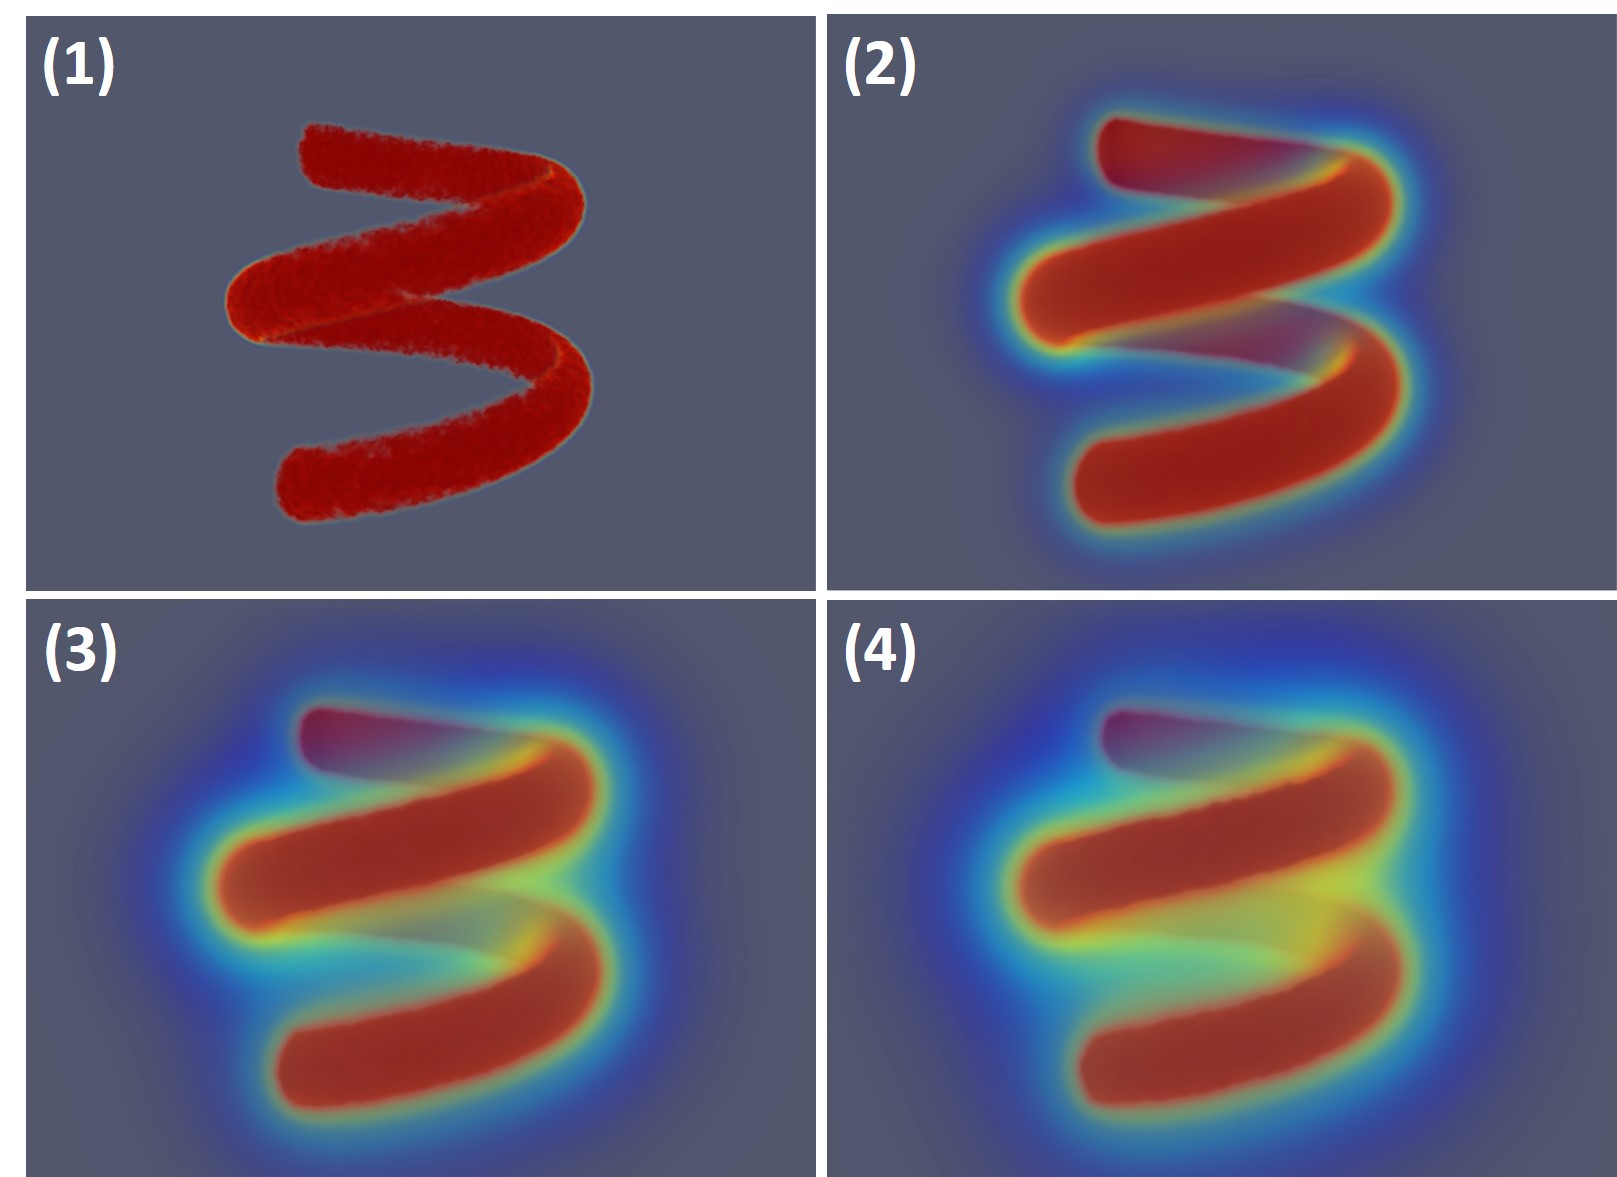
\includegraphics[width=12cm]{logo_degradation}
\caption{Simulation result of the logo example.} \label{fig:logo_degradation}
\end{figure}

\subsubsection{Example 3 - biodegradation of a cuboid}\label{sec:example3}

The aim of this example is to show how one can combine the approaches taken in the last two examples and use the UI to generate the execution command so that it can be used to run the model in another environment from command line. The idea is simple: \biodeg{}-UI writes the run command and the output of the core model in the ``Output'' panel, so we can have the execution command if we setup the simulation, run it, stop it immediately, and have a look at the ``Output'' panel.

For demonstrating this, we simulate the degradation of a cuboid inside a cubic container. The mesh file is called \verb|cuboid.mesh|, which has $\num{830808}$ elements. The mesh labels for scaffold and medium are the same as the default values on the \biodeg{}-UI (1 for scaffold and 2 for medium), so we don't need to change them. The setup will be straightforward since we just need to adjust the input and output, but the UI will generate a command with a full list of arguments, making it easy to modify it later if required.

Start the UI,
make sure \menu[,]{Geometry \& Mesh, Import external mesh} is checked, click the browse button in front of the ``File'' box (\menu[,]{Geometry \& Mesh, Import mesh, File}), navigate to the \verb|demo| directory, and select the \verb|cuboid.mesh| file. Since we don't want to change anything else, go directory to the output settings, mark
 \menu[,]{Output, Output options, Write VTK output} (since we want to have graphical output for postprocessing), and specify the output directory by clicking on the browse button in front of the ``Output directory'' (\menu[,]{Output, Output options, Output directory}) and select a directory of desire. 
 
As the setup is over, we are ready to run the simulation. Click the \menu[,]{Run simulation} button, wait a moment for the command to appear in the ``Output'' panel (written  like \verb|Executing: <command>|) and then click \menu[,]{Stop simulation}. You can now copy the command from the ``Output'' panel by selecting it, right clicking on it, and choosing \verb|Copy|. For this sample case, the command looks like this:

\begin{verbatim}
$ mpiexec -n 3 FreeFem++-mpi BioDeg-core/src/main.edp -v 0 -import_mesh 1 
-mesh_file "/home/mojtaba/BioDeg/demo/cuboid.mesh" -label_scaffold 1 -label_medium 2 
-refine_initial_mesh 0  -material_density 0.001735 -film_density 0.002344 
-material_satur 0.000134 -material_eps 0.55 -material_tau 1 -k1 7 -k2 1e+10 -d_mg 0.05 
-d_cl 0.05 -d_oh 25 -initial_cl 5.17e-06 -initial_oh 1e-07 -solve_mg 1 -solve_film 1 
-solve_cl 1 -solve_oh 1 -solve_ls 1 -time_step 0.025 -final_time 21 -do_redistance 1  
-redistance_time 1 -solve_fluid 0 -write_fluid_output 0 -text_output_file 
"/home/mojtaba/BioDeg/cuboid_output/output.txt" -write_vtk 1 -vtk_output_name 
"/home/mojtaba/BioDeg/cuboid_output/output" -save_last_state 0 -save_each 0.25 
-output_per_area 0 -save_multiplier 1 -export_scaffold 0  -save_initial_mesh 0 
-save_initial_partitioned_mesh 0
\end{verbatim}

More details of these parameters can be found in Section \hyperref[sec:index]{Index}. You can always omit the parameters with the default value, resulting in a command like the one we made in the second example (Section~\ref{sec:example2}).

\subsection{Postprocessing of the results using ParaView} \label{sec:postprocess}

Although the \biodeg{}-UI provides some basic postprocessing features such as the total amount of mass loss (via clicking on \menu[,]{Plot mass loss data} which reads the output text file) and a couple of ParaView templates (via selecting one of the variables on \menu[,]{Graphical output} and clicking \menu[,]{View results}), it can always  be beneficial to visualize the results the way you want. Doing this enables you to reproduce the demonstration you see in Figs.~\ref{fig:screw_degradation} and \ref{fig:logo_degradation} as well as any plot output you want, such as plotting variables over a line.

The details of the postprocessing steps of \biodeg{} results are discussed in the following YouTube videos, describing how to use ParaView to visualize the degrading scaffold beside plotting other output variables such as film formation and pH changes:

\begin{itemize}
\item 
\url{https://www.youtube.com/watch?v=yeBPGwP3L80&ab_channel=TuxRiders}
\item
\url{https://www.youtube.com/watch?v=Sz-eBML2pxs&ab_channel=TuxRiders}
\end{itemize}

The following videos gives you an idea on how to plot the values of different variables over a line and how to do some quantitative analysis on the results:

\begin{itemize}
\item 
\url{https://www.youtube.com/watch?v=tGi-jk2UE2U&ab_channel=TuxRiders}
\end{itemize}

For visualizing the fluid flow, more advanced techniques should be used. The following videos demonstrates how to visualize the fluid field around a degrading object simulated by \biodeg{}:

\begin{itemize}
\item
\url{https://www.youtube.com/watch?v=CByh84hOslU&ab_channel=TuxRiders}
\item
\url{https://www.youtube.com/watch?v=Xzwe94bvGJI&ab_channel=TuxRiders}
\end{itemize}

\section{Future extensions to \biodeg}
\label{sec:future}
The future versions of BioDeg will focus on implementing the following methodologies/features.
\begin{itemize}
\item Extending the core models to capture more complex chemistry of biodegradation by considering more reactions occurring in buffered solutions.

\item Adding support for more base materials like Fe and Zn.

\item Considering the effect of alloying elements and complex compositions.

\item Adding more post-processing features to \biodeg{} UI.

\item Adding basic visualization to \biodeg{} UI using ParaView Glance.

\item Improving the performance of fluid flow solver by employing a gradient-based solver.

\item Considering GPU support by enabling GPU computing in recent versions of PETSc.

\end{itemize} 


\section{Finding answers to more questions}
\label{sec:questions-and-answers}
If you have questions that go beyond this manual, there are several
resources you may refer to:
\begin{itemize}
\item For questions/suggestions about \biodeg{} installation, bugs, or similar stuff please use the 
	\href{https://github.com/mbarzegary/BioDeg/issues}{\biodeg{} issue tracker}. 

\item \biodeg{} is primarily based on the \href{http://www.freefem.org/}{FreeFEM}. If you have particular questions about FreeFEM, contact the community at \url{https://community.freefem.org/}.

\item If you have specific questions about \biodeg{} that are not suitable
  for public and archived mailing lists, you can contact the
  primary developer and mentor:
  \begin{itemize}
  \item Mojtaba Barzegari: \url{mojtaba.barzegari@kuleuven.be}.
  \item Liesbet Geris: \url{liesbet.geris@kuleuven.be} (Mentor).
  \end{itemize}
\end{itemize}


\appendix

\section{Run-time input parameters}
\label{sec:parameters}
The underlying description of the input parameters also includes a ``Standard/Advanced'' label, which signifies whether an input parameter is a standard one or an advanced level parameter. The default values of the ``Advanced'' parameters are good enough for almost all cases. However, in some cases user may need to use ``Advanced'' labeled parameters. For user convenience, all input parameters are also indexed at the end of this manual in Section \hyperref[sec:index]{Index}.
\subsection{Geometry and mesh parameters}
\label{parameters:mesh}

\begin{itemize}

\item {\it Parameter name:} {\tt import\_mesh}
\phantomsection
\label{parameters:import_mesh}

\index[prmindex]{refine\_initial\_mesh}
\index[prmindexfull]{Geometry and mesh!import mesh}

{\it Default:} true (1)

{\it Description:} [Standard] Boolean parameter specifying whether an external mesh file is imported or a container box as well as a cubic scaffold would be created on the fly for simulation.

{\it Possible values:} A boolean value (1 or 0)

\item {\it Parameter name:} {\tt mesh\_file}
\phantomsection
\label{parameters:mesh_file}

\index[prmindex]{mesh\_file}
\index[prmindexfull]{Geometry and mesh!mesh file}

{\it Default:} Should be provided

{\it Description:} [Standard] Path to the input mesh file (in MEDIT {\tt .mesh} format), which can be either absolute or relative. Is relevant only if parameter {\tt import\_mesh} is set to TRUE.

{\it Possible values:} Any string value 


\item {\it Parameter name:} {\tt label\_scaffold}
\phantomsection
\label{parameters:label_scaffold}

\index[prmindex]{label\_scaffold}
\index[prmindexfull]{Geometry and mesh!label scaffold}

{\it Default:} 1

{\it Description:} [Standard] The label of the (volume) region supposed to be scaffold in the input mesh (can be viewed in programs like GMSH before importing into \biodeg{}). 

{\it Possible values:} Any positive integer value 


\item {\it Parameter name:} {\tt label\_medium}
\phantomsection
\label{parameters:label_medium}

\index[prmindex]{label\_medium}
\index[prmindexfull]{Geometry and mesh!label medium}

{\it Default:} 2 

{\it Description:} [Standard] The label of the (volume) region supposed to be the medium (electrolyte) in the input mesh.

{\it Possible values:} Any positive integer value 


\item {\it Parameter name:} {\tt label\_wall}
\phantomsection
\label{parameters:label_wall}

\index[prmindex]{label\_wall}
\index[prmindexfull]{Geometry and mesh!label wall}

{\it Default:} 3

{\it Description:} [Advanced] The label of the surface in the input mesh to be assigned as wall (no slip boundary condition) in the fluid flow simulations.

{\it Possible values:} Any positive integer value 


\item {\it Parameter name:} {\tt label\_inlet}
\phantomsection
\label{parameters:label_inlet}

\index[prmindex]{label\_inlet}
\index[prmindexfull]{Geometry and mesh!label inlet}

{\it Default:} 4

{\it Description:} [Advanced] The label of the surface in the input mesh to be assigned as flow inlet (constant velocity boundary condition) in the fluid flow simulations.

{\it Possible values:} Any positive integer value 


\item {\it Parameter name:} {\tt label\_outlet}
\phantomsection
\label{parameters:label_outlet}

\index[prmindex]{label\_outlet}
\index[prmindexfull]{Geometry and mesh!label outlet}

{\it Default:} 5

{\it Description:} [Advanced] The label of the surface in the input mesh to be assigned as flow outlet (zero pressure boundary condition) in the fluid flow simulations.

{\it Possible values:} Any positive integer value 


\item {\it Parameter name:} {\tt box\_length}
\phantomsection
\label{parameters:box_length}

\index[prmindex]{box\_length}
\index[prmindexfull]{Geometry and mesh!box length}

{\it Default:} 20.0

{\it Description:} [Standard] In case of {\tt import\_mesh} being FALSE, specifies the length of the container box (for the electrolyte) in mm.

{\it Possible values:} Any positive floating point number 


\item {\it Parameter name:} {\tt cube\_size\_x}
\phantomsection
\label{parameters:cube_size_x}

\index[prmindex]{cube\_size\_x}
\index[prmindexfull]{Geometry and mesh!cube size x}

{\it Default:} 13.0

{\it Description:} [Standard] In case of {\tt import\_mesh} being FALSE, specifies the length of the scaffold cuboid along the x axis in mm.

{\it Possible values:} Any positive floating point number 


\item {\it Parameter name:} {\tt cube\_size\_y}
\phantomsection
\label{parameters:cube_size_y}

\index[prmindex]{cube\_size\_y}
\index[prmindexfull]{Geometry and mesh!cube size y}

{\it Default:} 13.0

{\it Description:} [Standard] In case of {\tt import\_mesh} being FALSE, specifies the length of the scaffold cuboid along the y axis in mm.

{\it Possible values:} Any positive floating point number 


\item {\it Parameter name:} {\tt cube\_size\_z}
\phantomsection
\label{parameters:cube_size_z}

\index[prmindex]{cube\_size\_z}
\index[prmindexfull]{Geometry and mesh!cube size z}

{\it Default:} 4.0

{\it Description:} [Standard] In case of {\tt import\_mesh} being FALSE, specifies the length of the scaffold cuboid along the z axis in mm.


{\it Possible values:} Any positive floating point number 


\item {\it Parameter name:} {\tt mesh\_size}
\phantomsection
\label{parameters:mesh_size}

\index[prmindex]{mesh\_size}
\index[prmindexfull]{Geometry and mesh!mesh size}

{\it Default:} 32

{\it Description:} [Standard] Number of elements on each edge of the container box, so a higher number means a finer mesh. The mesh size of the cuboid will be adjusted accordingly or can be adaptively refined by setting parameter {\tt refine\_initial\_mesh} to TRUE.

{\it Possible values:} Any positive integer number 


\item {\it Parameter name:} {\tt refine\_initial\_mesh}
\phantomsection
\label{parameters:refine_initial_mesh}

\index[prmindex]{refine\_initial\_mesh}
\index[prmindexfull]{Geometry and mesh!refine initial mesh}

{\it Default:} false (0)

{\it Description:} [Advanced] A boolean parameter specifying if the mesh (no matter if imported or generated) should be adaptively refined on the metal-medium interface (corrosion surface). This affects the beginning of the simulation only (on the initial mesh).

{\it Possible values:} A boolean value (1 or 0)


\item {\it Parameter name:} {\tt mshmet\_error}
\phantomsection
\label{parameters:mshmet_error}

\index[prmindex]{mshmet\_error}
\index[prmindexfull]{Geometry and mesh!mshmet error}

{\it Default:} 0.01

{\it Description:} [Advanced] Since the open source tool {\tt mshmet} is used for creating a metric for refining the mesh on the level set signed distance function, a tolerance should be specified for it. A lower value results to a finer mesh.

{\it Possible values:} Any floating point number


\item {\it Parameter name:} {\tt mesh\_size\_min}
\phantomsection
\label{parameters:mesh_size_min}

\index[prmindex]{mesh\_size\_min}
\index[prmindexfull]{Geometry and mesh!mesh size min}

{\it Default:} 0.04

{\it Description:} [Advanced] Specifies the smallest element size to be passed to the {\tt tetgen} mesh generator for refining the initial mesh.

{\it Possible values:} Any floating point number


\item {\it Parameter name:} {\tt mesh\_size\_max}
\phantomsection
\label{parameters:mesh_size_max}

\index[prmindex]{mesh\_size\_max}
\index[prmindexfull]{Geometry and mesh!mesh size max}

{\it Default:} 0.8

{\it Description:} [Advanced] Specifies the largest element size to be passed to the {\tt tetgen} mesh generator for refining the initial mesh.

{\it Possible values:} Any floating point number

\end{itemize}



\subsection{Materials and boundary conditions parameters}
\label{parameters:material}

\begin{itemize}
\item {\it Parameter name:} {\tt material\_density}
\phantomsection
\label{parameters:material_density}

\index[prmindex]{material\_density}
\index[prmindexfull]{Materials and boundary conditions!material density}

{\it Default:} 1.735e-3

{\it Description:} [Standard] 

{\it Possible values:} Any floating point number


\item {\it Parameter name:} {\tt film\_density}
\phantomsection
\label{parameters:film_density}

\index[prmindex]{film\_density}
\index[prmindexfull]{Materials and boundary conditions!film density}

{\it Default:} 2.3446e-3

{\it Description:} [Standard] 

{\it Possible values:} Any floating point number


\item {\it Parameter name:} {\tt material\_satur}
\phantomsection
\label{parameters:material_satur}

\index[prmindex]{material\_satur}
\index[prmindexfull]{Materials and boundary conditions!material satur}

{\it Default:} 0.134e-3

{\it Description:} [Advanced] 

{\it Possible values:} Any floating point number


\item {\it Parameter name:} {\tt material\_eps}
\phantomsection
\label{parameters:material_eps}

\index[prmindex]{material\_eps}
\index[prmindexfull]{Materials and boundary conditions!material eps}

{\it Default:} 0.55

{\it Description:} [Advanced] 

{\it Possible values:} Any floating point number between 0 and 1


\item {\it Parameter name:} {\tt material\_tau}
\phantomsection
\label{parameters:material_tau}

\index[prmindex]{material\_tau}
\index[prmindexfull]{Materials and boundary conditions!material tau}

{\it Default:} 1.0

{\it Description:} [Advanced] 

{\it Possible values:} Any floating point number


\item {\it Parameter name:} {\tt d\_mg}
\phantomsection
\label{parameters:d_mg}

\index[prmindex]{d\_mg}
\index[prmindexfull]{Materials and boundary conditions!d mg}

{\it Default:} 0.05

{\it Description:} [Standard] 

{\it Possible values:} Any floating point number


\item {\it Parameter name:} {\tt d\_cl}
\phantomsection
\label{parameters:d_cl}

\index[prmindex]{d\_cl}
\index[prmindexfull]{Materials and boundary conditions!d cl}

{\it Default:} 0.05

{\it Description:} [Standard] 

{\it Possible values:} Any floating point number


\item {\it Parameter name:} {\tt d\_oh}
\phantomsection
\label{parameters:d_oh}

\index[prmindex]{d\_oh}
\index[prmindexfull]{Materials and boundary conditions!d oh}

{\it Default:} 25.2

{\it Description:} [Standard] 

{\it Possible values:} Any floating point number


\item {\it Parameter name:} {\tt k1}
\phantomsection
\label{parameters:k1}

\index[prmindex]{k1}
\index[prmindexfull]{Materials and boundary conditions!k1}

{\it Default:} 7.0

{\it Description:} [Standard] 

{\it Possible values:} Any floating point number


\item {\it Parameter name:} {\tt k2}
\phantomsection
\label{parameters:k2}

\index[prmindex]{k2}
\index[prmindexfull]{Materials and boundary conditions!k2}

{\it Default:} 1e15

{\it Description:} [Standard] 

{\it Possible values:} Any floating point number


\item {\it Parameter name:} {\tt fluid\_nu}
\phantomsection
\label{parameters:fluid_nu}

\index[prmindex]{fluid\_nu}
\index[prmindexfull]{Materials and boundary conditions!fluid nu}

{\it Default:} 0.85

{\it Description:} [Advanced] 

{\it Possible values:} Any floating point number


\item {\it Parameter name:} {\tt fluid\_in\_x}
\phantomsection
\label{parameters:fluid_in_x}

\index[prmindex]{fluid\_in\_x}
\index[prmindexfull]{Materials and boundary conditions!fluid in x}

{\it Default:} 0.1

{\it Description:} [Advanced] 

{\it Possible values:} Any floating point number


\item {\it Parameter name:} {\tt fluid\_in\_y}
\phantomsection
\label{parameters:fluid_in_y}

\index[prmindex]{fluid\_in\_y}
\index[prmindexfull]{Materials and boundary conditions!fluid in y}

{\it Default:} 0

{\it Description:} [Advanced] 

{\it Possible values:} Any floating point number


\item {\it Parameter name:} {\tt fluid\_in\_z}
\phantomsection
\label{parameters:fluid_in_z}

\index[prmindex]{fluid\_in\_z}
\index[prmindexfull]{Materials and boundary conditions!fluid in z}

{\it Default:} 0

{\it Description:} [Advanced] 

{\it Possible values:} Any floating point number


\item {\it Parameter name:} {\tt initial\_cl}
\phantomsection
\label{parameters:initial_cl}

\index[prmindex]{initial\_cl}
\index[prmindexfull]{Materials and boundary conditions!initial cl}

{\it Default:} 5.175e-6

{\it Description:} [Standard] 

{\it Possible values:} Any floating point number


\item {\it Parameter name:} {\tt initial\_oh}
\phantomsection
\label{parameters:initial_oh}

\index[prmindex]{initial\_oh}
\index[prmindexfull]{Materials and boundary conditions!initial oh}

{\it Default:} 1e-7

{\it Description:} [Standard] 

{\it Possible values:} Any floating point number


\end{itemize}



\subsection{Solver parameters}
\label{parameters:sovler}

\begin{itemize}
\item {\it Parameter name:} {\tt solve\_mg}
\phantomsection
\label{parameters:solve_mg}

\index[prmindex]{solve\_mg}
\index[prmindexfull]{Solver!solve mg}

{\it Default:} true (1)

{\it Description:} [Standard] Boolean parameter indicating whether the equation for material dissolution and ions release should be solved or not. This equation is the most essential equation and in most use-cases should be solved.

{\it Possible values:} Any boolean value (1 or 0)


\item {\it Parameter name:} {\tt solve\_film}
\phantomsection
\label{parameters:solve_film}

\index[prmindex]{solve\_film}
\index[prmindexfull]{Solver!solve film}

{\it Default:} true (1)

{\it Description:} [Standard] Boolean parameter indicating whether the equation for the protective film formation should be solved or not.

{\it Possible values:} Any boolean value (1 or 0)


\item {\it Parameter name:} {\tt solve\_cl}
\phantomsection
\label{parameters:solve_cl}

\index[prmindex]{solve\_cl}
\index[prmindexfull]{Solver!solve cl}

{\it Default:} true (1)

{\it Description:} [Standard] Boolean parameter indicating whether the equation for the transport of chloride ions should be solved or not.

{\it Possible values:} Any boolean value (1 or 0)


\item {\it Parameter name:} {\tt solve\_oh}
\phantomsection
\label{parameters:solve_oh}

\index[prmindex]{solve\_oh}
\index[prmindexfull]{Solver!solve oh}

{\it Default:} true (1)

{\it Description:} [Standard] Boolean parameter indicating whether the equation for the transport of hydroxide ions should be solved or not. This equation is essential for calculating the pH changes, if desired.

{\it Possible values:} Any boolean value (1 or 0)


\item {\it Parameter name:} {\tt solve\_ls}
\phantomsection
\label{parameters:solve_ls}

\index[prmindex]{solve\_ls}
\index[prmindexfull]{Solver!solve ls}

{\it Default:} true (1)

{\it Description:} [Standard] Boolean parameter indicating whether the level set surface tracking equation should be solved or not. Surface tracking is essential for computing the mass loss.

{\it Possible values:} Any boolean value (1 or 0)


\item {\it Parameter name:} {\tt solve\_fluid}
\phantomsection
\label{parameters:solve_fluid}

\index[prmindex]{solve\_fluid}
\index[prmindexfull]{Solver!solve fluid}

{\it Default:} false (0)

{\it Description:} [Standard] Boolean parameter indicating whether the fluid flow equation should be solved or not.

{\it Possible values:} Any boolean value (1 or 0)


\item {\it Parameter name:} {\tt solve\_full\_ns}
\phantomsection
\label{parameters:solve_full_ns}

\index[prmindex]{solve\_full\_ns}
\index[prmindexfull]{Solver!solve full ns}

{\it Default:} true (1)

{\it Description:} [Advanced] Boolean parameter specifying which fluid flow equation to solve: the full transient Navier-Stokes equations or a steady-state Stokes equation. A true value (1) results in \biodeg{} solving the former equation.

{\it Possible values:} Any boolean value (1 or 0)


\item {\it Parameter name:} {\tt write\_fluid\_output}
\phantomsection
\label{parameters:write_fluid_output}

\index[prmindex]{write\_fluid\_output}
\index[prmindexfull]{Solver!write fluid output}

{\it Default:} true (1)

{\it Description:} [Advanced] Boolean parameter specifying whether the fluid flow quantities (velocity field components and pressure) should be saved in the output VTK file or not. Requires {\tt write\_vtk} be TRUE.

{\it Possible values:} Any boolean value (1 or 0)


\item {\it Parameter name:} {\tt solve\_fluid\_each}
\phantomsection
\label{parameters:solve_fluid_each}

\index[prmindex]{solve\_fluid\_each}
\index[prmindexfull]{Solver!solve fluid each}

{\it Default:} 10

{\it Description:} [Advanced] Determines the number of time steps to skip before solving the specified fluid flow equation. For example, if the value is set to 10 (default value), the fluid equation gets solved in time steps 1, 11, 21, \ldots.

{\it Possible values:} Any positive integer number


\item {\it Parameter name:} {\tt time\_step}
\phantomsection
\label{parameters:time_step}

\index[prmindex]{time\_step}
\index[prmindexfull]{Solver!time step}

{\it Default:} 0.025

{\it Description:} [Advanced] The time step value for the numerical schemes of the simulations.

{\it Possible values:} Any floating point number


\item {\it Parameter name:} {\tt final\_time}
\phantomsection
\label{parameters:final_time}

\index[prmindex]{final\_time}
\index[prmindexfull]{Solver!final time}

{\it Default:} 21.0

{\it Description:} [Standard] 

{\it Possible values:} Any floating point number


\item {\it Parameter name:} {\tt do\_redistance}
\phantomsection
\label{parameters:do_redistance}

\index[prmindex]{do\_redistance}
\index[prmindexfull]{Solver!do redistance}

{\it Default:} true (1)

{\it Description:} [Advanced] 

{\it Possible values:} Any boolean value (1 or 0)


\item {\it Parameter name:} {\tt redistance\_time}
\phantomsection
\label{parameters:redistance_time}

\index[prmindex]{redistance\_time}
\index[prmindexfull]{Solver!redistance time}

{\it Default:} 1.0

{\it Description:} [Advanced] 

{\it Possible values:} Any floating point number

\end{itemize}


\subsection{Output parameters}
\label{parameters:output}

\begin{itemize}
\item {\it Parameter name:} {\tt text\_output\_file}
\phantomsection
\label{parameters:text_output_file}

\index[prmindex]{text\_output\_file}
\index[prmindexfull]{Output!text output file}

{\it Default:} "output/result.txt"

{\it Description:} [Standard] 

{\it Possible values:} Any string value referring to a valid path


\item {\it Parameter name:} {\tt write\_vtk}
\phantomsection
\label{parameters:write_vtk}

\index[prmindex]{write\_vtk}
\index[prmindexfull]{Output!write vtk}

{\it Default:} true (1)

{\it Description:} [Standard] 

{\it Possible values:} Any boolean value (1 or 0)


\item {\it Parameter name:} {\tt vtk\_output\_name}
\phantomsection
\label{parameters:vtk_output_name}

\index[prmindex]{vtk\_output\_name}
\index[prmindexfull]{Output!vtk output name}

{\it Default:} "output/output"

{\it Description:} [Standard] 

{\it Possible values:} Any string value referring to a valid path


\item {\it Parameter name:} {\tt save\_each}
\phantomsection
\label{parameters:save_each}

\index[prmindex]{save\_each}
\index[prmindexfull]{Output!save each}

{\it Default:} 0.25

{\it Description:} [Standard] 

{\it Possible values:} Any floating point number


\item {\it Parameter name:} {\tt save\_last\_state}
\phantomsection
\label{parameters:save_last_state}

\index[prmindex]{save\_last\_state}
\index[prmindexfull]{Output!save last state}

{\it Default:} true (1)

{\it Description:} [Standard] 

{\it Possible values:} Any boolean value (1 or 0)


\item {\it Parameter name:} {\tt output\_per\_area}
\phantomsection
\label{parameters:output_per_area}

\index[prmindex]{output\_per\_area}
\index[prmindexfull]{Output!output per area}

{\it Default:} false (0)

{\it Description:} [Advanced] 

{\it Possible values:} Any boolean value (1 or 0)


\item {\it Parameter name:} {\tt save\_multiplier}
\phantomsection
\label{parameters:save_multiplier}

\index[prmindex]{save\_multiplier}
\index[prmindexfull]{Output!save multiplier}

{\it Default:} 1.0

{\it Description:} [Advanced] 

{\it Possible values:} Any floating point number


\item {\it Parameter name:} {\tt export\_scaffold}
\phantomsection
\label{parameters:export_scaffold}

\index[prmindex]{export\_scaffold}
\index[prmindexfull]{Output!export scaffold}

{\it Default:} false (0)

{\it Description:} [Advanced] 

{\it Possible values:} Any boolean value (1 or 0)


\item {\it Parameter name:} {\tt export\_scaffold\_each}
\phantomsection
\label{parameters:export_scaffold_each}

\index[prmindex]{export\_scaffold\_each}
\index[prmindexfull]{Output!export scaffold each}

{\it Default:} 1.0

{\it Description:} [Advanced] 

{\it Possible values:} Any floating point number


\item {\it Parameter name:} {\tt export\_scaffold\_volume}
\phantomsection
\label{parameters:export_scaffold_volume}

\index[prmindex]{export\_scaffold\_volume}
\index[prmindexfull]{Output!export scaffold volume}

{\it Default:} true (1)

{\it Description:} [Advanced] 

{\it Possible values:} Any boolean value (1 or 0)


\item {\it Parameter name:} {\tt export\_scaffold\_surface}
\phantomsection
\label{parameters:export_scaffold_surface}

\index[prmindex]{export\_scaffold\_surface}
\index[prmindexfull]{Output!export scaffold surface}

{\it Default:} true (1)

{\it Description:} [Advanced] 

{\it Possible values:} Any boolean value (1 or 0)


\item {\it Parameter name:} {\tt save\_initial\_mesh}
\phantomsection
\label{parameters:save_initial_mesh}

\index[prmindex]{save\_initial\_mesh}
\index[prmindexfull]{Output!save initial mesh}

{\it Default:} false (0)

{\it Description:} [Advanced] 

{\it Possible values:} Any boolean value (1 or 0)


\item {\it Parameter name:} {\tt save\_initial\_partitioned\_mesh}
\phantomsection
\label{parameters:save_initial_partitioned_mesh}

\index[prmindex]{save\_initial\_partitioned\_mesh}
\index[prmindexfull]{Output!save initial partitioned mesh}

{\it Default:} false (0)

{\it Description:} [Advanced] 

{\it Possible values:} Any boolean value (1 or 0)


\end{itemize}



\pagebreak


\indexprologue{The following is a listing of all run-time parameters, sorted
  by the section in which they appear. 
  \addcontentsline{toc}{section}{\numberline{}Index of run-time parameters with
    section names}
  \label{sec:runtime-parameter-index-full}
}
\printindex[prmindexfull]

\end{document}
